\documentclass [norsk,a4paper,twoside]{article}\usepackage[]{graphicx}\usepackage[]{color}
%% maxwidth is the original width if it is less than linewidth
%% otherwise use linewidth (to make sure the graphics do not exceed the margin)
\makeatletter
\def\maxwidth{ %
  \ifdim\Gin@nat@width>\linewidth
    \linewidth
  \else
    \Gin@nat@width
  \fi
}
\makeatother

\definecolor{fgcolor}{rgb}{0.345, 0.345, 0.345}
\newcommand{\hlnum}[1]{\textcolor[rgb]{0.686,0.059,0.569}{#1}}%
\newcommand{\hlstr}[1]{\textcolor[rgb]{0.192,0.494,0.8}{#1}}%
\newcommand{\hlcom}[1]{\textcolor[rgb]{0.678,0.584,0.686}{\textit{#1}}}%
\newcommand{\hlopt}[1]{\textcolor[rgb]{0,0,0}{#1}}%
\newcommand{\hlstd}[1]{\textcolor[rgb]{0.345,0.345,0.345}{#1}}%
\newcommand{\hlkwa}[1]{\textcolor[rgb]{0.161,0.373,0.58}{\textbf{#1}}}%
\newcommand{\hlkwb}[1]{\textcolor[rgb]{0.69,0.353,0.396}{#1}}%
\newcommand{\hlkwc}[1]{\textcolor[rgb]{0.333,0.667,0.333}{#1}}%
\newcommand{\hlkwd}[1]{\textcolor[rgb]{0.737,0.353,0.396}{\textbf{#1}}}%
\let\hlipl\hlkwb

\usepackage{framed}
\makeatletter
\newenvironment{kframe}{%
 \def\at@end@of@kframe{}%
 \ifinner\ifhmode%
  \def\at@end@of@kframe{\end{minipage}}%
  \begin{minipage}{\columnwidth}%
 \fi\fi%
 \def\FrameCommand##1{\hskip\@totalleftmargin \hskip-\fboxsep
 \colorbox{shadecolor}{##1}\hskip-\fboxsep
     % There is no \\@totalrightmargin, so:
     \hskip-\linewidth \hskip-\@totalleftmargin \hskip\columnwidth}%
 \MakeFramed {\advance\hsize-\width
   \@totalleftmargin\z@ \linewidth\hsize
   \@setminipage}}%
 {\par\unskip\endMakeFramed%
 \at@end@of@kframe}
\makeatother

\definecolor{shadecolor}{rgb}{.97, .97, .97}
\definecolor{messagecolor}{rgb}{0, 0, 0}
\definecolor{warningcolor}{rgb}{1, 0, 1}
\definecolor{errorcolor}{rgb}{1, 0, 0}
\newenvironment{knitrout}{}{} % an empty environment to be redefined in TeX

\usepackage{alltt}
\addtolength{\hoffset}{-0.5cm}
\addtolength{\textwidth}{1cm}
\addtolength{\voffset}{-1cm}
\addtolength{\textheight}{2cm}


%for nice looking tabs
\usepackage{booktabs}

\usepackage[norsk]{babel}
\usepackage[utf8x]{inputenc}
\usepackage{textcomp}
\usepackage{fancyhdr}
\pagestyle{fancy}
\usepackage{amsmath}
\usepackage{rotating} %add rotating for plain tables
\usepackage{pdflscape} %add rotating/landcape for pdf

%add rotating for plain tables
\usepackage{rotating}

%add rotating/landcape for pdf
\usepackage{pdflscape}

%bytte font
\renewcommand{\familydefault}{\sfdefault}

%setter grå skrift fremfort sort
\usepackage{xcolor}
\usepackage{graphicx}
\usepackage[pdftex, colorlinks, linkcolor=OffBlaa3, urlcolor=OffBlaa3]{hyperref}
\IfFileExists{upquote.sty}{\usepackage{upquote}}{}
\begin{document}








\section{Oppsummeringstall for NKR}

% latex table generated in R 3.4.1 by xtable 1.8-2 package
% Wed Aug 23 15:08:31 2017
\begin{table}[ht]
\centering
\begin{tabular}{lrrrrrr}
  \hline
 & 2012 & 2013 & 2014 & 2015 & 2016 & Sum \\ 
  \hline
Ahus & 50 & 151 & 67 & 136 & 184 & 605 \\ 
  Aleris, Bergen & 217 & 265 & 145 & 95 & 59 & 939 \\ 
  Aleris, Oslo & 152 & 4 & 38 & 190 & 72 & 773 \\ 
  Arendal & 84 & 95 & 87 & 82 & 72 & 558 \\ 
  Bodø & 5 & 0 & 0 & 27 & 20 & 88 \\ 
  Bærum & 79 & 88 & 65 & 111 & 134 & 612 \\ 
  Drammen & 148 & 102 & 186 & 249 & 273 & 1108 \\ 
  Elverum & 94 & 127 & 147 & 139 & 128 & 887 \\ 
  Flekkefjord & 12 & 10 & 2 & 8 & 6 & 53 \\ 
  Førde & 0 & 0 & 0 & 0 & 25 & 32 \\ 
  Gjøvik & 85 & 74 & 94 & 75 & 118 & 643 \\ 
  Haugesund & 5 & 38 & 54 & 42 & 82 & 221 \\ 
  Haukeland, nevrokir & 158 & 170 & 186 & 168 & 170 & 1001 \\ 
  Haukeland, ort & 4 & 0 & 1 & 18 & 23 & 50 \\ 
  Ibsensykehuset & 0 & 0 & 0 & 0 & 1 & 1 \\ 
  Kolibri Medical Group & 0 & 18 & 3 & 0 & 0 & 21 \\ 
  Kristiansand & 96 & 112 & 110 & 137 & 165 & 788 \\ 
  Kristiansund & 0 & 0 & 0 & 0 & 34 & 34 \\ 
  Kysthospitalet Hagevik & 202 & 244 & 269 & 275 & 291 & 1698 \\ 
  Larvik & 29 & 0 & 0 & 0 & 117 & 202 \\ 
  Levanger & 75 & 99 & 112 & 116 & 109 & 659 \\ 
  Lillehammer & 91 & 61 & 62 & 99 & 77 & 511 \\ 
  Martina Hansens & 319 & 270 & 304 & 341 & 307 & 2006 \\ 
  Namsos & 64 & 55 & 93 & 73 & 71 & 430 \\ 
  NIMI & 27 & 24 & 129 & 111 & 116 & 458 \\ 
  Oslofjordklinikken Vest & 0 & 0 & 6 & 59 & 96 & 161 \\ 
  Oslofjordklinikken Øst & 266 & 303 & 345 & 341 & 324 & 1943 \\ 
  Rana & 10 & 19 & 23 & 23 & 30 & 145 \\ 
  Rikshospitalet, nevrokir & 37 & 52 & 55 & 63 & 33 & 400 \\ 
  Rikshospitalet, ort & 15 & 4 & 2 & 0 & 0 & 22 \\ 
  Skien & 1 & 23 & 41 & 39 & 66 & 170 \\ 
  St.Olavs, nevrokir & 345 & 325 & 346 & 356 & 299 & 2259 \\ 
  St.Olavs, ort & 58 & 46 & 50 & 32 & 39 & 350 \\ 
  Stavanger, nevrokir & 212 & 200 & 172 & 156 & 131 & 979 \\ 
  Stavanger, ort & 231 & 234 & 237 & 274 & 270 & 1331 \\ 
  Teres Colloseum, Oslo & 5 & 41 & 26 & 26 & 79 & 192 \\ 
  Teres Colloseum, Stavanger & 0 & 0 & 31 & 46 & 32 & 159 \\ 
  Teres, Bergen & 0 & 0 & 0 & 0 & 0 & 15 \\ 
  Teres, Drammen & 43 & 37 & 0 & 0 & 0 & 138 \\ 
  Ullevål, nevrokir & 34 & 80 & 30 & 42 & 88 & 274 \\ 
  Ullevål, ort & 117 & 136 & 126 & 162 & 166 & 955 \\ 
  Ulriksdal & 92 & 9 & 0 & 0 & 0 & 338 \\ 
  UNN, nevrokir & 275 & 221 & 222 & 245 & 206 & 1759 \\ 
  Volda & 24 & 29 & 27 & 38 & 31 & 170 \\ 
  Volvat & 0 & 21 & 80 & 139 & 136 & 377 \\ 
  Østfold & 0 & 0 & 61 & 48 & 44 & 153 \\ 
  Ålesund & 105 & 103 & 127 & 102 & 109 & 747 \\ 
  Sum & 3866 & 3890 & 4161 & 4683 & 4833 & 27415 \\ 
   \hline
\end{tabular}
\caption{Antall registreringer ved hver avdeling siste 5 år, samt totalt siden 2010.} 
\label{tab:AntReg}
\end{table}


Tabell \ref{tab:AntReg} viser antall 
registreringer gjort ved de respektive avdelinger hvert år. Vi ser at det er  
47 avdelinger som registrerer og at det i perioden 2010 til 2016 totalt er registrert 27415 
operasjoner. Av disse er 53.1\% utført på menn og 46.9\% på kvinner.
Siste inngrep registrert i datauttrekket som ligger til grunn for denne rapporten, ble utført 
2016-12-30. 
\par 
\clearpage



\section{Bakgrunnsdata}
\subsection{Alder}

Gjennomsnittsalderen har økt jevnt fra 53.7 år i 2010 til 56.0 år i 2016. 
Ryggkirurgi øker mest i den eldste og mest sårbare delen av
befolkningen. Disse pasientene vet vi at trenger mer omfattende utredning og
lengre liggetid. Dette medfører økte kostnader, spesielt for offentlige sykehus som i
all hovedsak håndterer denne pasientgruppen. I 2016 ble 23.3 \% (1120 operasjoner) av alle
ryggoperasjonene meldt til NKR utført på personer over 70 år.

\textit{Evt. figur med tidstrend av andel over 70 år..?}




Figur \ref{fig:Alder} viser aldersfordeling for alle pasienter i 2016.


\begin{figure}[ht]
	\centering 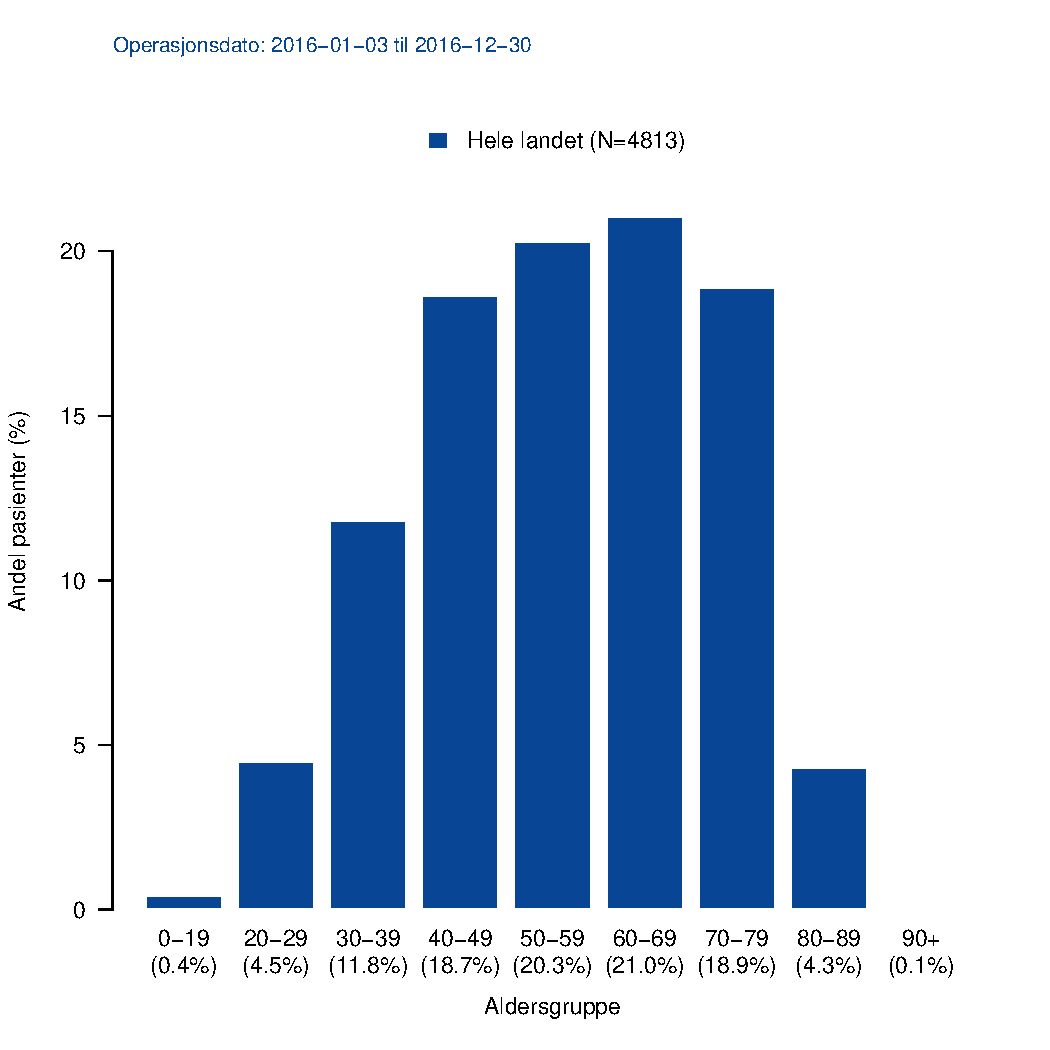
\includegraphics[width= 0.8\textwidth]{FigAlderFord.pdf}
	\caption{\label{fig:Alder} Aldersfordeling., 2016}
\end{figure}





%\begin{figure}[ht]
%	\centering 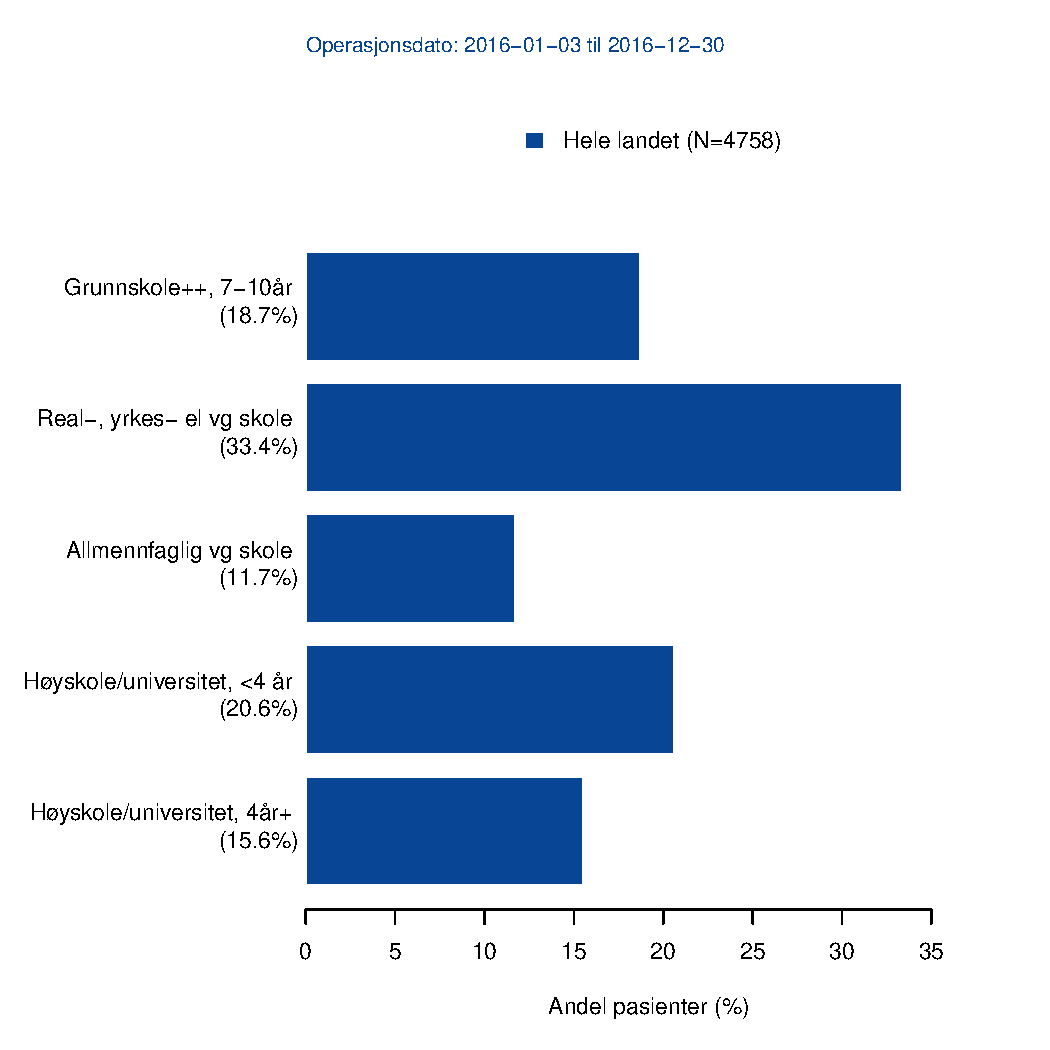
\includegraphics[width= figKrymp1\textwidth]{FigUtd.pdf}
%	\caption{\label{fig:Utd} Andel ryggoperasjoner utført på personer som er 70 år eller mer.}}
%\end{figure}

Figur 3.3: Andel ryggoperasjoner utført på personer som er 70 år eller mer.
\textit{Trenger ny figurtype (AndelTid) for å lage denne} \\
\textbf{I møtet 29.mai, ble det anbefalt å fjerne fig. 3.3-6 og bare kommentere resultatene.}


\subsection{Morsmål / etnisitet}

% latex table generated in R 3.4.1 by xtable 1.8-2 package
% Wed Aug 23 15:08:31 2017
\begin{table}[ht]
\centering
\begin{tabular}{lrr}
  \hline
 & Antall & Andeler \\ 
  \hline
Norsk & 4509 & 93.7\% \\ 
  Samisk & 5 & 0.1\% \\ 
  Annet & 277 & 5.8\% \\ 
  Ikke svart & 22 & 0.5\% \\ 
   \hline
\end{tabular}
\caption{Pasientenes morsmål} 
\label{tab:Morsm}
\end{table}


Tabell \ref{tab:Morsm} viser fordeling av norske, samiske og andre fremmedsåpråklige pasienter.
Andel fremmedspråklige 
pasienter (inkl. samisk) var 5.9\% . 


\subsection{Utdanning}
Figur \ref{fig:Utd} viser nivå av utdanning 
Opplysningene om utdanning er rapportert av pasientene selv.



\begin{figure}[ht]
	\centering 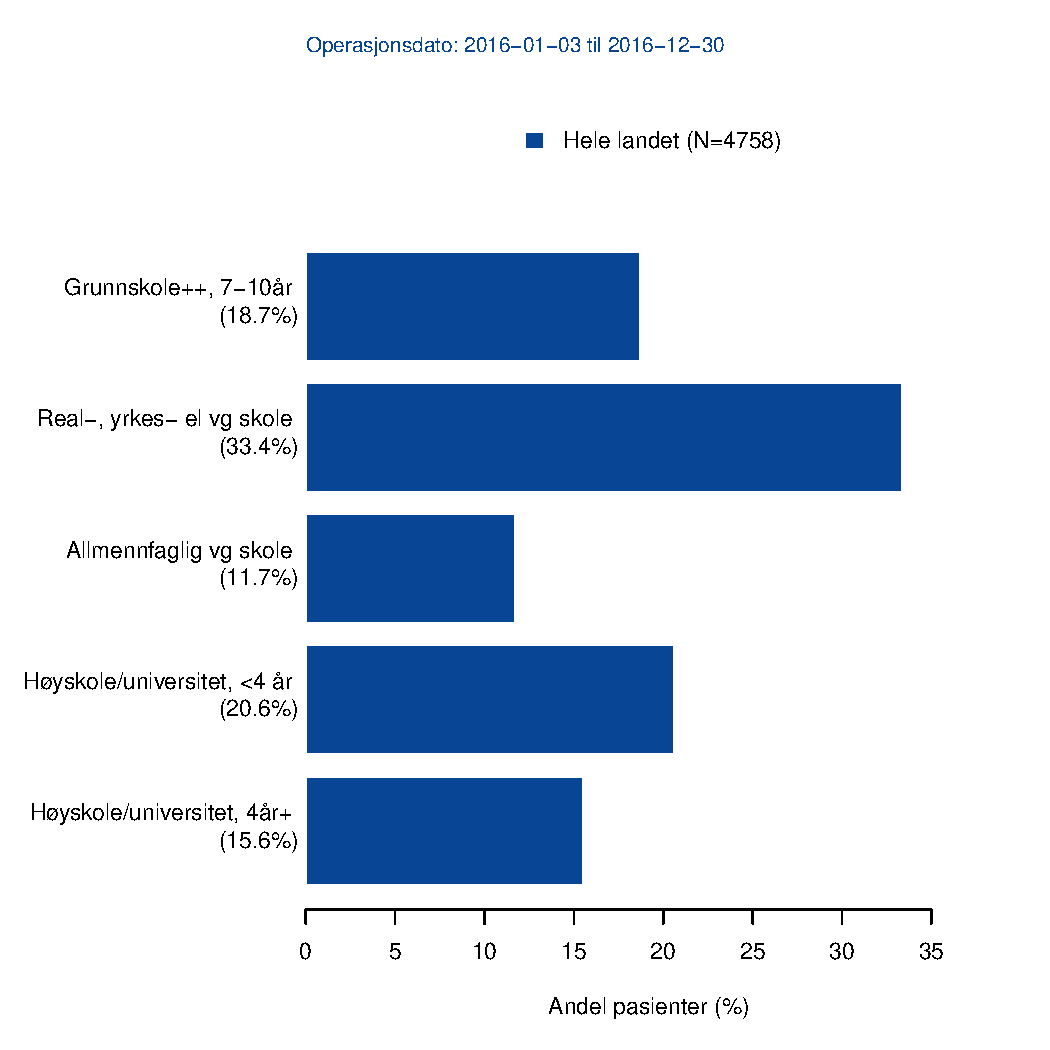
\includegraphics[width= 0.8\textwidth]{FigUtd.pdf}
	\caption{\label{fig:Utd} Høyeste fullførte utdanning.}
\end{figure}




\subsection{Arbeidsstatus}

% latex table generated in R 3.4.1 by xtable 1.8-2 package
% Wed Aug 23 15:08:31 2017
\begin{table}[ht]
\centering
\begin{tabular}{lr}
  \hline
 & Andeler \\ 
  \hline
I arbeid & 19.2\% \\ 
  Hjemmeværende & 1.6\% \\ 
  Student/skoleelev & 1.2\% \\ 
  Pensjonist & 28.8\% \\ 
  Arbeidsledig & 1.4\% \\ 
  Sykemeldt & 22.9\% \\ 
  Aktiv sykemeldt & 1.1\% \\ 
  Delvis Sykemeldt & 7.9\% \\ 
  Attføring/rehabiliteirng & 4.2\% \\ 
  Uføretrygdet & 11.6\% \\ 
   \hline
\end{tabular}
\caption{Arbeidsstatus, pasienter operert i 2016} 
\label{tab:Arb}
\end{table}


Tabell \ref{tab:Arb} viser fordeling av arbeidsstatus før operasjon for de 98.1\% 
av pasientene som har svart på spørsmål om arbeidsstatus.
Andelen pasienter som mottok sykepenger (sykemeldte, uføretrygdede eller personer 
på attføring) og av den grunn var helt eller delvis ute av jobb før operasjonen var 
47.7 \%. 
Median varighet av sykemelding/attføring/rehabilitering  før operasjon var 
15 uker.


\clearpage


\subsection{Uføretrygd og erstatning }

Tabell \ref{tab:Ufor} viser pasientenes svar på spørsmålet: ``Har du søkt om uføretrygd?''.

% latex table generated in R 3.4.1 by xtable 1.8-2 package
% Wed Aug 23 15:08:31 2017
\begin{table}[ht]
\centering
\begin{tabular}{lr}
  \hline
 & Andeler \\ 
  \hline
Ja & 2\% \\ 
  Nei & 75.2\% \\ 
  Planlegger å søke & 2.2\% \\ 
  Er innvilget & 11.5\% \\ 
  Ikke besvart & 9.1\% \\ 
   \hline
\end{tabular}
\caption{Spørsmål: Har du søkt om uføretrygd?} 
\label{tab:Ufor}
\end{table}



Tabell \ref{tab:Erst} viser pasientenes svar på spørsmålet: ``Har du søkt om erstatning?'' 

% latex table generated in R 3.4.1 by xtable 1.8-2 package
% Wed Aug 23 15:08:31 2017
\begin{table}[ht]
\centering
\begin{tabular}{lr}
  \hline
 & Andeler \\ 
  \hline
Ja & 2.6\% \\ 
  Nei & 87.6\% \\ 
  Planlegger å søke & 1.8\% \\ 
  Er innvilget & 2.1\% \\ 
  Ikke besvart & 5.9\% \\ 
   \hline
\end{tabular}
\caption{Spørsmål: Har du søkt om erstatning fra forsikringsselskap eller folketrygden, 
		eventuelt yrkesskadeerstatning)?} 
\label{tab:Erst}
\end{table}



\subsection{Tidligere ryggoperert}
Informasjonen er hentet fra legeskjema.
Figur \ref{fig:TidlOp} viser en prosentvis fordelig mellom primæroperasjon, det vil si første gangs 
operasjon, og operasjoner hos pasienter som har vært operert tidligere.  
Søylene representerer hvert år frem til i dag. Tallet på toppen av søylen viser antall operasjoner utført 
det aktuelle året.



\begin{figure}[ht]
	\centering 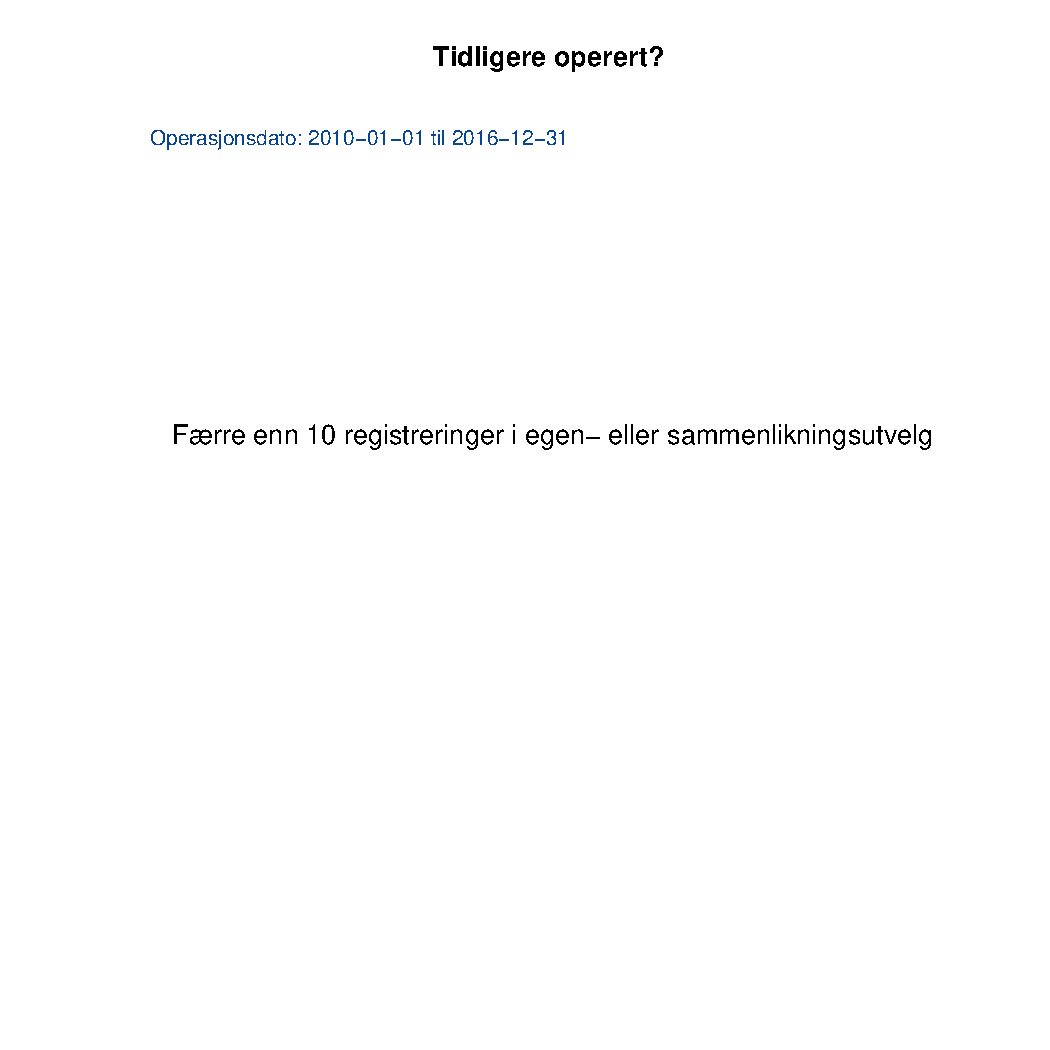
\includegraphics[width= 0.8\textwidth]{TidlOp.pdf}
	\caption{\label{fig:TidlOp} Tidligere operert? }
\end{figure}



Av de pasientene operert i 2016 som hadde vært operert tidligere, var 61.0982212\% 
operert i samme nivå, 33.4880124\% 
operert i annet nivå og 5.4137664\% 
operert i både samme og annet nivå. 


\subsection{Kroppsmasseindex (Body Mass Index, BMI)}



Opplysninger om høyde og vekt er rapportert fra pasientene selv.
Andelen pasienter med fedme har vært jevt økende fra 18.6 \%
til 24.5 \%
Figur \ref{fig:BMI} viser fordeling av BMI for alle pasienter i 2016. 

\begin{figure}[ht]
	\centering 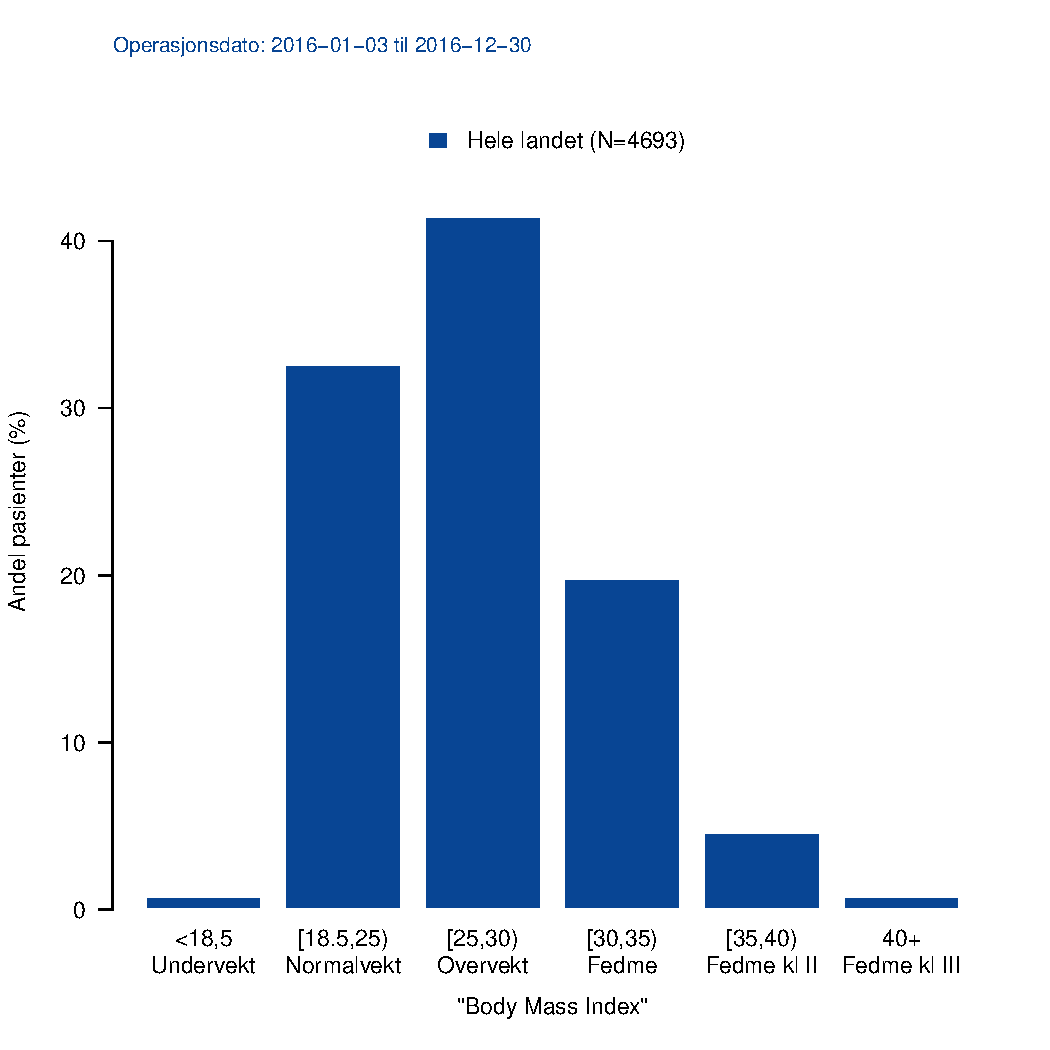
\includegraphics[width= 0.8\textwidth]{FigBMI.pdf}
	\caption{\label{fig:BMI} Pasientenes BMI (Body Mass Index).}
\end{figure}



\clearpage


\subsection{Varighet av smerter i rygg-/hofte og av utstrålende smerter på operasjonstidspunktet}

% latex table generated in R 3.4.1 by xtable 1.8-2 package
% Wed Aug 23 15:08:33 2017
\begin{table}[ht]
\centering
\begin{tabular}{lr}
  \hline
 & Andeler \\ 
  \hline
Ingen rygg-/hoftesmerter & 1.7\% \\ 
  $<$ 3 mnd & 9\% \\ 
  3 - 12 mnd & 30.8\% \\ 
  1 - 2 år & 16.5\% \\ 
  $>$ 2 år & 38.2\% \\ 
  Ikke besvart & 3.8\% \\ 
   \hline
\end{tabular}
\caption{Varighet av rygg-/hoftesmerter på operasjonstidspunktet} 
\label{tab:SmRH}
\end{table}
% latex table generated in R 3.4.1 by xtable 1.8-2 package
% Wed Aug 23 15:08:33 2017
\begin{table}[ht]
\centering
\begin{tabular}{lr}
  \hline
 & Andeler \\ 
  \hline
Ingen utstrålende smerter & 2.7\% \\ 
  $<$ 3 mnd & 13.5\% \\ 
  3 - 12 mnd & 35\% \\ 
  1 - 2 år & 17.5\% \\ 
  $>$ 2 år & 26.2\% \\ 
  Ikke besvart & 5.2\% \\ 
   \hline
\end{tabular}
\caption{Varighet av nåværende utstrålende smerter} 
\label{tab:Utstr}
\end{table}

Spørsmålene er besvart av pasienten.
Tabellene \ref{tab:SmRH}  og \ref{tab:Utstr} (vises også senere...) viser fordeling av hvor lenge pasientene har hatt 
hhv. smerter i rygg/hofte og utstrålende smerter. Figur \ref{fig:VarighSmerteUtstrAvd} viser hvor stor andel av prolapspasienter som har hatt ustrålende smerter i mer enn ett år ved hvert sykehus. Figur \ref{fig:VarighSmerteRyggAvd} viser prolapspasienter med som har hatt smerter i rygg-/hofte i mer enn ett år før operasjon.

\textbf{Kommer tilsvarende figurer på spinalstenose...}



\begin{figure}[h] 
  \scalebox{0.8}{\includegraphics{VarighUtstrAvd.pdf}}
  \caption{Prolapspasienter som har utstrålende smerter
			i mer enn ett år før operasjonen.}
  \label{fig:VarighSmerteUtstrAvd}
\end{figure}

\begin{figure}[h] 
  \scalebox{0.8}{\includegraphics{VarighRyggHofAvd.pdf}}
  \caption{Prolapspasienter som har hatt smerter i rygg-/hofte
			i mer enn ett år før operasjonen.}
  \label{fig:VarighSmerteRyggAvd}
\end{figure}


\textit{Tekst som tidligere var plassert i omtale av kvalitetsindikatorene... )}

\textbf{Effektiv håndtering (rett tid)}

I nasjonale retningslinjer (2007) er det anbefalt å operere pasienter for prolaps før
bensmertene har vart for lenge, helst innen 6-8 måneder. Derfor bør
pasientgruppen håndteres raskt og effektivt når beslutning om operasjon er tatt og
ikke-kirurgisk behandling har vært forsøkt. Data fra NKR og nyere forskning viser at
pasienter som opereres for prolaps og har hatt bensmerter mer enn ett år har
dårligere prognose. Andelen pasienter med bensmerter mer enn ett år på
operasjonstidspunkt var uendret fra 2010 til 2016 (47\%).
Figur 7 viser at det er stor variasjon i varighet av bensmerter hos pasienter som blir
operert ved ulike sykehus. Det har sannsynligvis sammenheng med ventetid for
utredning og operasjon og tilgjengelig operasjonskapasitet i forhold til etterspørsel.





\subsection{ASA-grad og røyking}
ASA angir pasientens ”sårbarhet” i forhold til å få anestesi og operasjon på en skala fra 1 til 5. 
Opplysningene skal hentes fra anestesiskjema som fylles ut av anestesilege/sykepleier før operasjon.
% latex table generated in R 3.4.1 by xtable 1.8-2 package
% Wed Aug 23 15:08:33 2017
\begin{table}[ht]
\centering
\begin{tabular}{crr}
  \hline
 & Antall & Prosent \\ 
  \hline
I & 1334 & 27.7\% \\ 
  II & 2787 & 57.9\% \\ 
  III & 657 & 13.7\% \\ 
  IV & 5 & 0.1\% \\ 
  Ikke besvart & 30 & 0.6\% \\ 
   \hline
\end{tabular}
\caption{Fordeling av ASA-grad, operasjoner utført i 2016} 
\label{tab:ASA}
\end{table}


Tabell \ref{tab:ASA} viser fordeling av ASA grad. Andelen pasienter med ASA grad I-II 
var 85.6\%. Pasienter som røyker, havner automatisk i ASA-grad II eller høyere. 
Det er 21\% av mennene og 22\% av kvinnene som røyker. 
Total andel røykere er 21\%



Det er 21\% av mennene og 22\% av kvinnene som røyker. 
Total andel røykere er 21\%





\subsection{Radiologisk utredning}

% latex table generated in R 3.4.1 by xtable 1.8-2 package
% Wed Aug 23 15:08:33 2017
\begin{table}[ht]
\centering
\begin{tabular}{lrr}
  \hline
 & Antall & Andeler \\ 
  \hline
CT & 339 & 7\% \\ 
  MR & 4712 & 97.9\% \\ 
  Radikulografi & 33 & 0.7\% \\ 
  Diskografi & 2 & 0\% \\ 
  Diagnostisk blokade & 12 & 0.2\% \\ 
  Røntgen LS-columna & 1043 & 21.7\% \\ 
  Med fleksjon/ekstensjon & 335 & 7\% \\ 
  Tot. ant. & 4813 &   \\ 
   \hline
\end{tabular}
\caption{Radiologisk vurdering, 2016} 
\label{tab:RV}
\end{table}


Tabell \ref{tab:RV} viser hvor stor andel av pasientene som har vært til ulike typer 
radiologisk undersøkelse. 
Spørsmålene er besvart av leger. En pasient kan ha vært til flere undersøkelser.




% latex table generated in R 3.4.1 by xtable 1.8-2 package
% Wed Aug 23 15:08:33 2017
\begin{table}[ht]
\centering
\begin{tabular}{lrr}
  \hline
 & Antall & Andeler \\ 
  \hline
Skiveprolaps & 2206 & 45.8\% \\ 
  Sentral spinalstenose & 1498 & 31.1\% \\ 
  Lateral spinalstenose & 1578 & 32.8\% \\ 
  Foraminal stenose & 590 & 12.3\% \\ 
  Degenerativ rygg/skivedegenerasjon & 767 & 15.9\% \\ 
  Istmisk spondylolistese & 146 & 3\% \\ 
  Degenerativ spondylolistese & 414 & 8.6\% \\ 
  Degenerativ skoliose & 125 & 2.6\% \\ 
  Synovial syste & 92 & 1.9\% \\ 
  Pseudomeningocele & 1 & 0\% \\ 
  Tot.ant. & 4813 &   \\ 
   \hline
\end{tabular}
\caption{Radiologiske diagnoser, 2016} 
\label{tab:RF}
\end{table}


Tabell \ref{tab:RF} viser diagnoser basert på radiologiske funn hos alle pasienter 
i 2016. 
Spørsmålene er besvart av leger.
En pasient kan ha flere diagnoser/radiologiske funn.
``Normalt'' er registrert som eneste billedfunn hos 1 pasient(er).
      ``Normal'' kan ikke være eneste billedfunn, så eventuelle registreringer skyldes sannsynligvis 
      feil/unøyaktig registrering.



\clearpage

\section{Virksomhetsdata}

\subsection{Type operasjon}

Figur \ref{fig:HovedInngrep} viser fordeling av hovedinngrep av hver type.
De nøyaktige tallene for antall registrerte operasjoner for hvert hovedinngrep 
framgår av Tabell \ref{tab:AntHovedInngrep}. \\
\textbf{Vi ble enige om å ta bort tabellen og beholde figuren, men det er kanskje bedre å heller beholde tabellen?}

% latex table generated in R 3.4.1 by xtable 1.8-2 package
% Wed Aug 23 15:08:34 2017
\begin{table}[ht]
\centering
\begin{tabular}{lrr}
  \hline
 & Antall & Andeler \\ 
  \hline
Udefinerbart & 127 & 2.6\% \\ 
  Prolapskirurgi & 2065 & 42.9\% \\ 
  Foramenotomi & 1816 & 37.7\% \\ 
  Laminektomi & 196 & 4.1\% \\ 
  Interspin. implantat & 0 & 0\% \\ 
  Fusjonskirurgi & 545 & 11.3\% \\ 
  Skiveprotese & 32 & 0.7\% \\ 
  Rev. av implantat & 32 & 0.7\% \\ 
   \hline
\end{tabular}
\caption{Fordeling av hovedinngrep, 2016} 
\label{tab:AntHovedInngrep}
\end{table}



\begin{figure}[ht]
	\centering 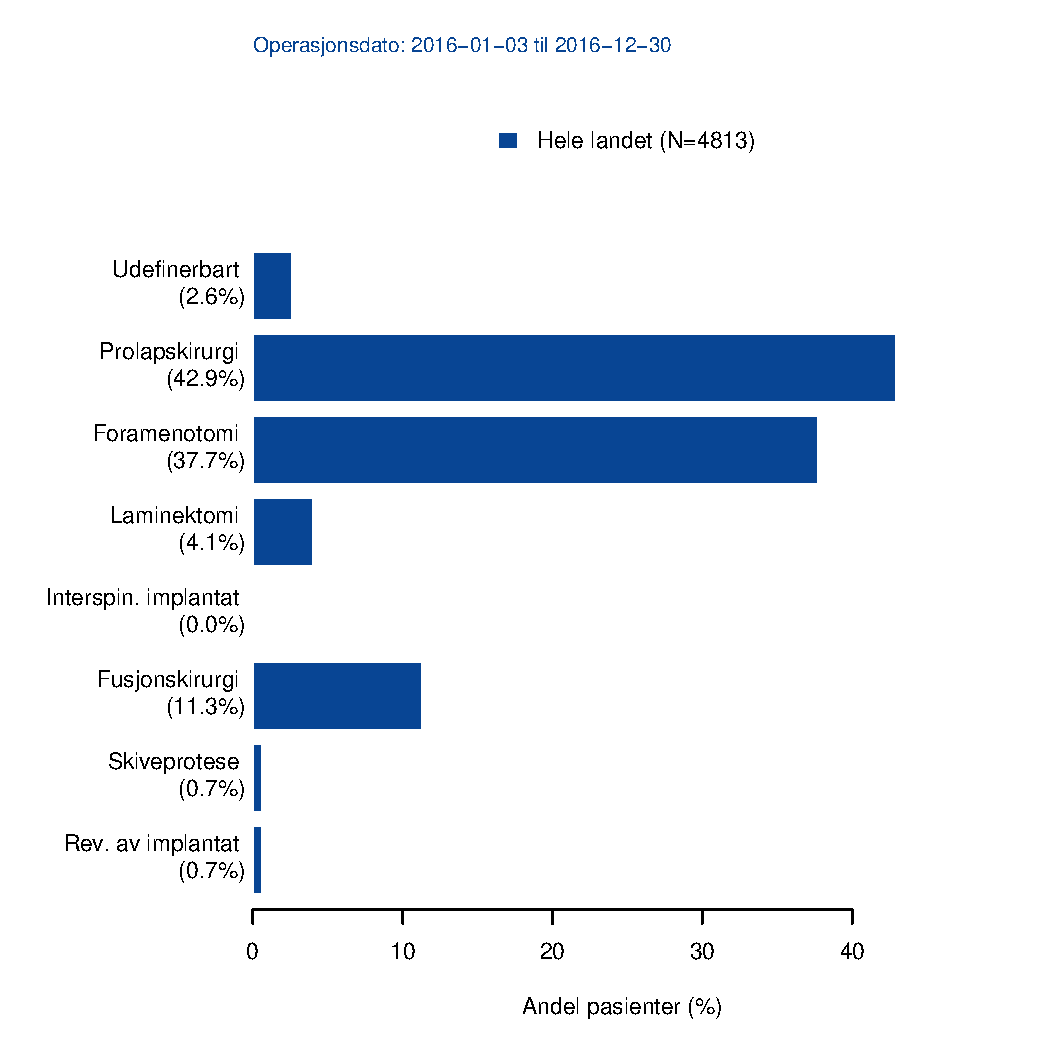
\includegraphics[width= 0.8\textwidth]{HovedInngrep.pdf}
	\caption{\label{fig:HovedInngrep} Hovedinngrep.}
\end{figure}




\subsection{Liggetid}

Informasjonen er hentet fra legeskjema.
Figur \ref{fig:Liggedogn} viser liggedøgnsfordeling for pasienter operert i 2016. Figur \ref{fig:LiggedognTid} viser gjennomsnittlig antall liggedøgn per år.  




\begin{figure}[h] 
\centerline{
  \scalebox{0.8}{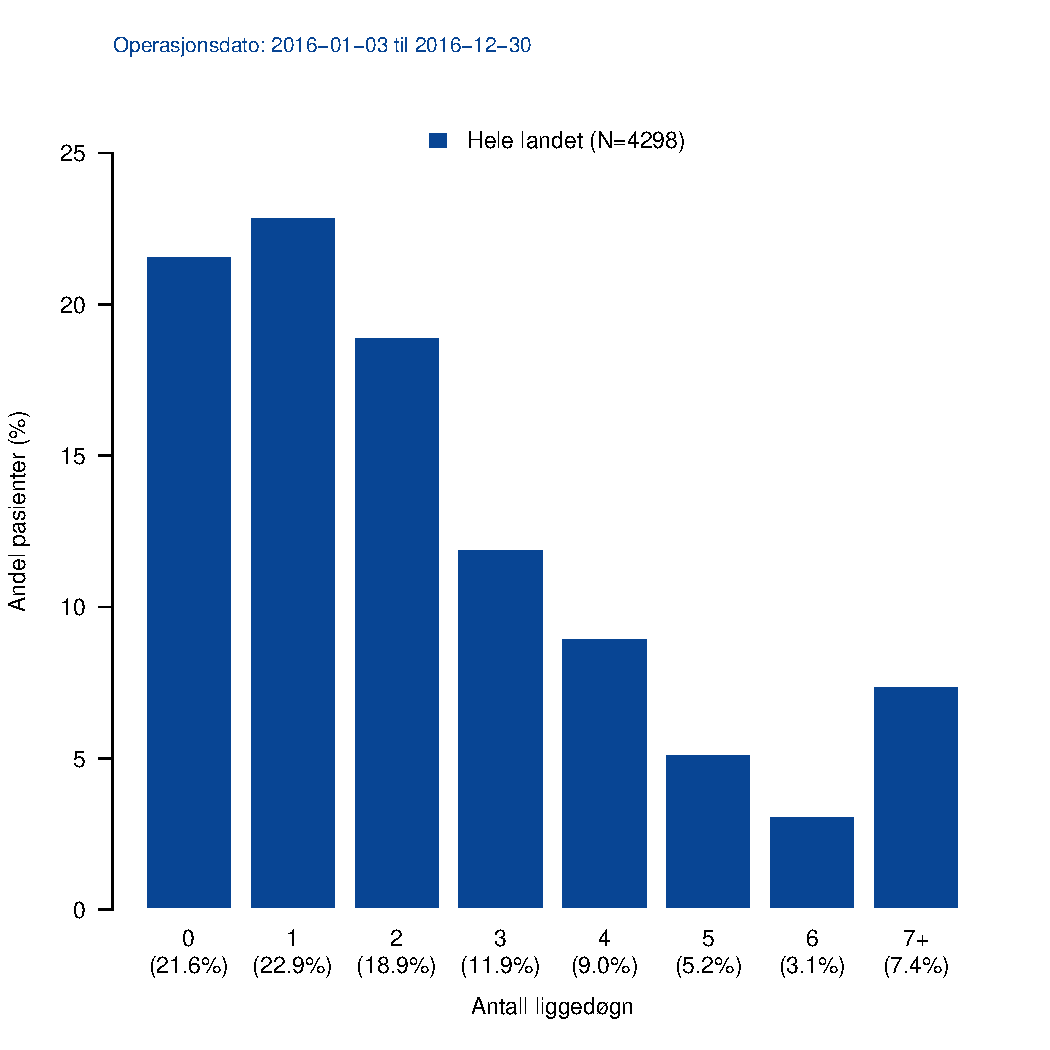
\includegraphics{FigLiggetidFord.pdf}}
  }
  \caption{Liggetid ved operasjon.}
  \label{fig:Liggedogn}
\end{figure}

\begin{figure}[h] 
\centerline{
  \scalebox{0.5}{\includegraphics{LiggetidBox.pdf}}
  \scalebox{0.5}{\includegraphics{LiggetidBox.pdf}}
  }
  \caption{Her kommer to figurer med liggetidstrend for hhv. prolaps og spinal stenose}
  \label{fig:LiggedognTid}
\end{figure}







\clearpage

\section{Resultatmål}
All informasjon i dette kapitlet er hentet fra pasientskjema. Ingen av resultatmålene er justert
for eventuelle ulikheter i pasientpopulasjonene.


\subsection{Effekt av operasjon kontra prescore}
Figur \ref{fig:EndrPre} viser sammenhengen mellom prescore og endring i de ulike effektmålene.





\subsection{Oswestry Disability Index (ODI)}
ODI er en score for fysisk funksjon og et sykdomsspesifikt livskvalitetsmål. Skalaen går fra 0
til 100, hvor 0 angir ingen funksjonshemming og følgelig beste livskvalitet.
Figur \ref{fig:OswEndr} viser fordeling av ODI før og etter operasjon.
Figur \ref{fig:OswEndrSml} viser andel pasienter med klinisk signifikant forbedring av ODI (dvs. minst 30$\%$) 12 måneder etter operasjon. Høyre del av figuren viser gjennomsnittlig endring 12 måneder etter operasjon sammenliknet med landet for øvrig og de tre avdelingene/sykehusene som har 
med størst forbedring i ODI. Merk at resultatene \textit{ikke} er justert for forskjeller i pasientpopulasjonene.




 

\begin{figure}[h] 
\centerline{
  \scalebox{0.8}{\includegraphics{OswEndrProlaps.pdf}}
  }
  \caption{jennomsnittlig endring i Oswestry for prolaps, ett år etter operasjon. Kommer tilsvarende figur for spinal stenose}}
  \label{fig:OswEndr}
\end{figure}




\clearpage


\subsection{Opplevd nytte av operasjon}

Figur \ref{fig:Nytte} viser hvor stor nytte pasientene opplever å ha hatt av behandlingen ett år etter operasjon fordelt på år. Det hvite merket på søylene angir andel pasienter som angir at de har blitt ''Frisk'' eller ''Mye bedre'' i landet for øvrig . Tallet øverst på søyla angir antall pasienter som har svart. 
I figuren er det gjort følgende aggregering av svaralternativene i spørreskjemaet:
\begin{itemize}
	\item ''Frisk mye/bedre'' omfatter ''helt bra'' og ''mye bedre'' 
	\item ''Omtrent uendret'' omfatter ''litt bedre'', ''ingen endring'' og ''litt verre'' 
	\item ''Klart verre'' omfatter ''mye verre'' og ''verre enn noen gang før''
\end{itemize}



\begin{figure}[h] 
	\begin{center}
  \scalebox{0.5}{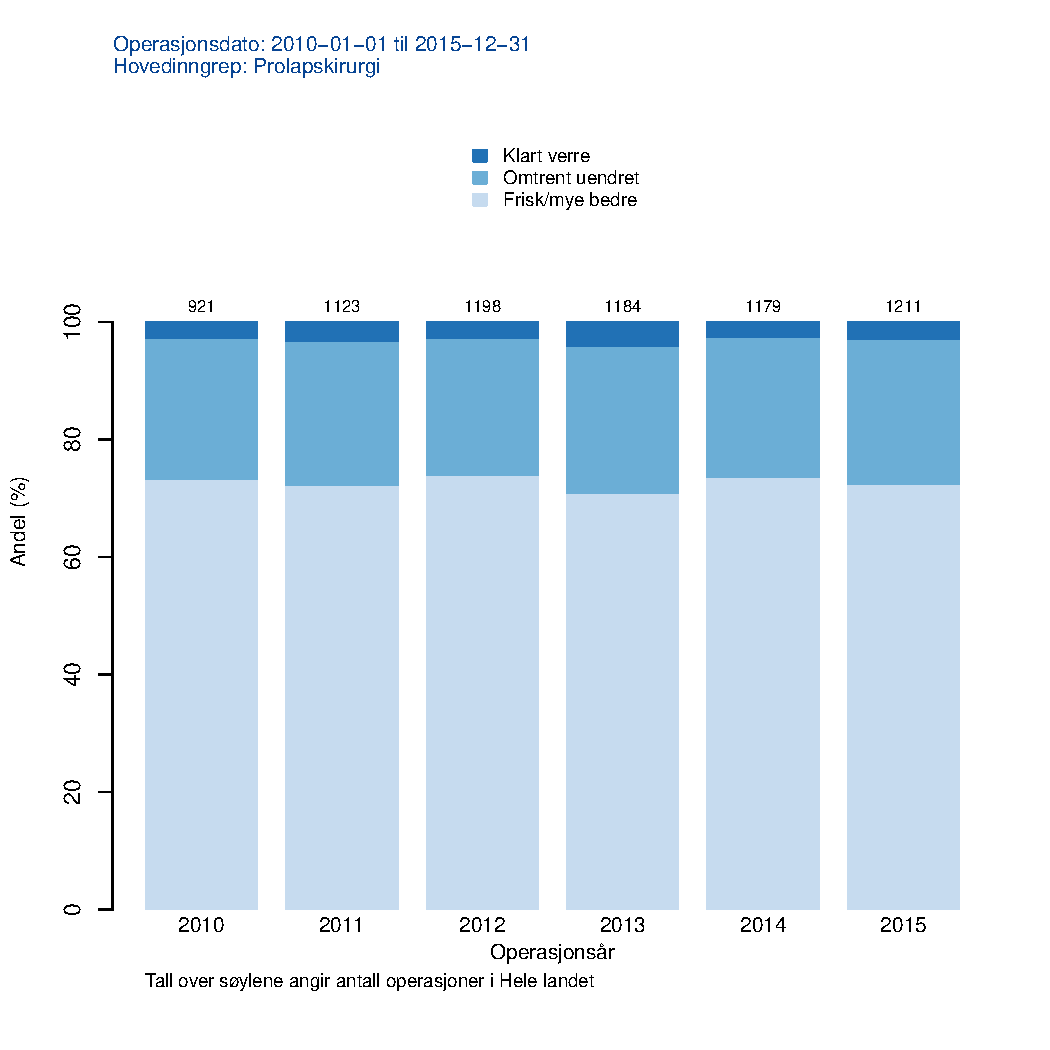
\includegraphics{FigNyttePro.pdf}}
  \scalebox{0.5}{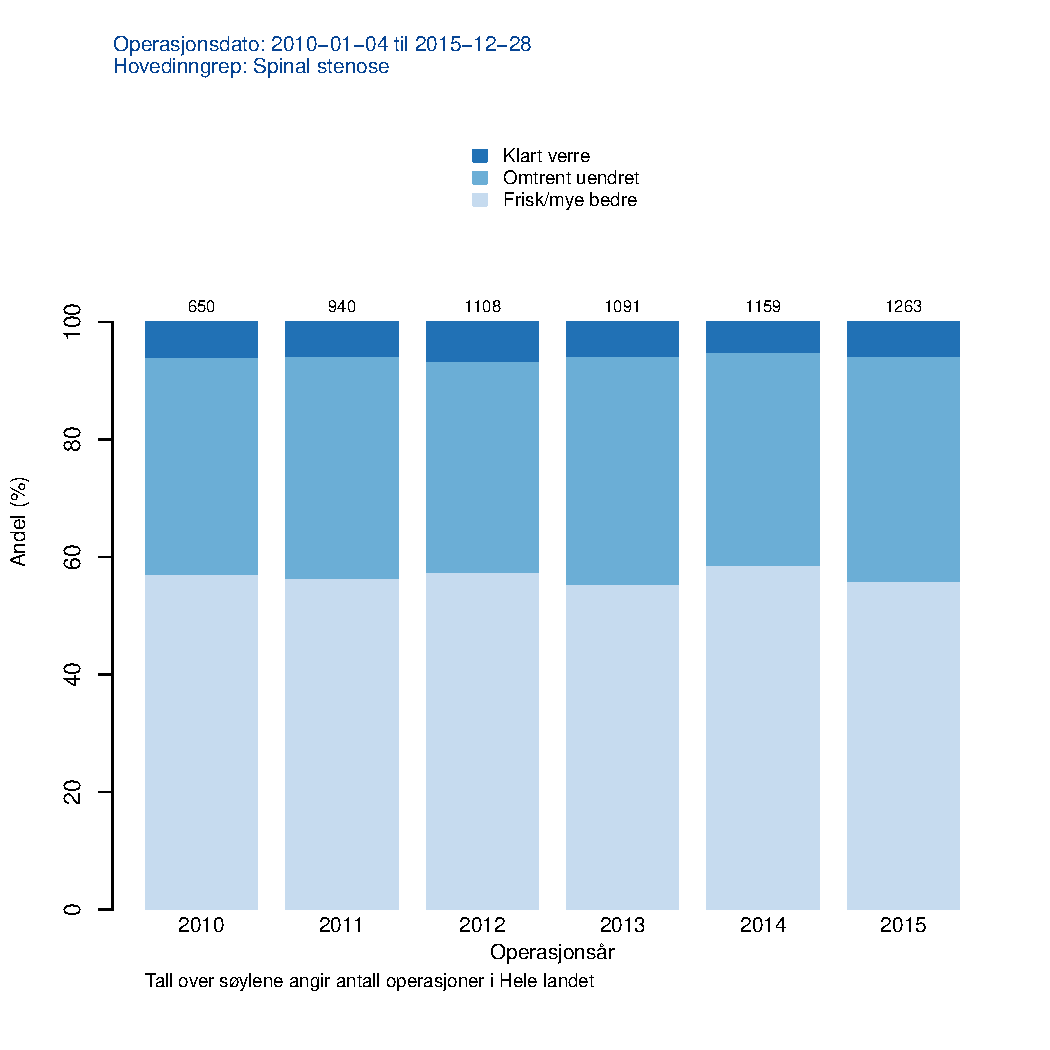
\includegraphics{FigNytteSS.pdf}}
	\end{center}
  \caption{Spørsmål stilt 12 måneder etter operasjon: Hvilken nytte mener du at du har hatt av operasjonen?}
  \label{fig:Nytte}
\end{figure}




\subsection{Pasienttilfredshet}

Figur \ref{fig:Fornoyd} viser hvor fornøyde pasientene er 12 mnd. 
etter operasjon fordelt på år. (\textbf{Her må det være feil i datagrunnlaget...} Det hvite merket på søylene angir andel fornøyde pasienter i landet for øvrig. Tallet øverst på søyla angir antall pasienter som har svart. 


\begin{figure}[h] 
	\begin{center}
\scalebox{0.5}{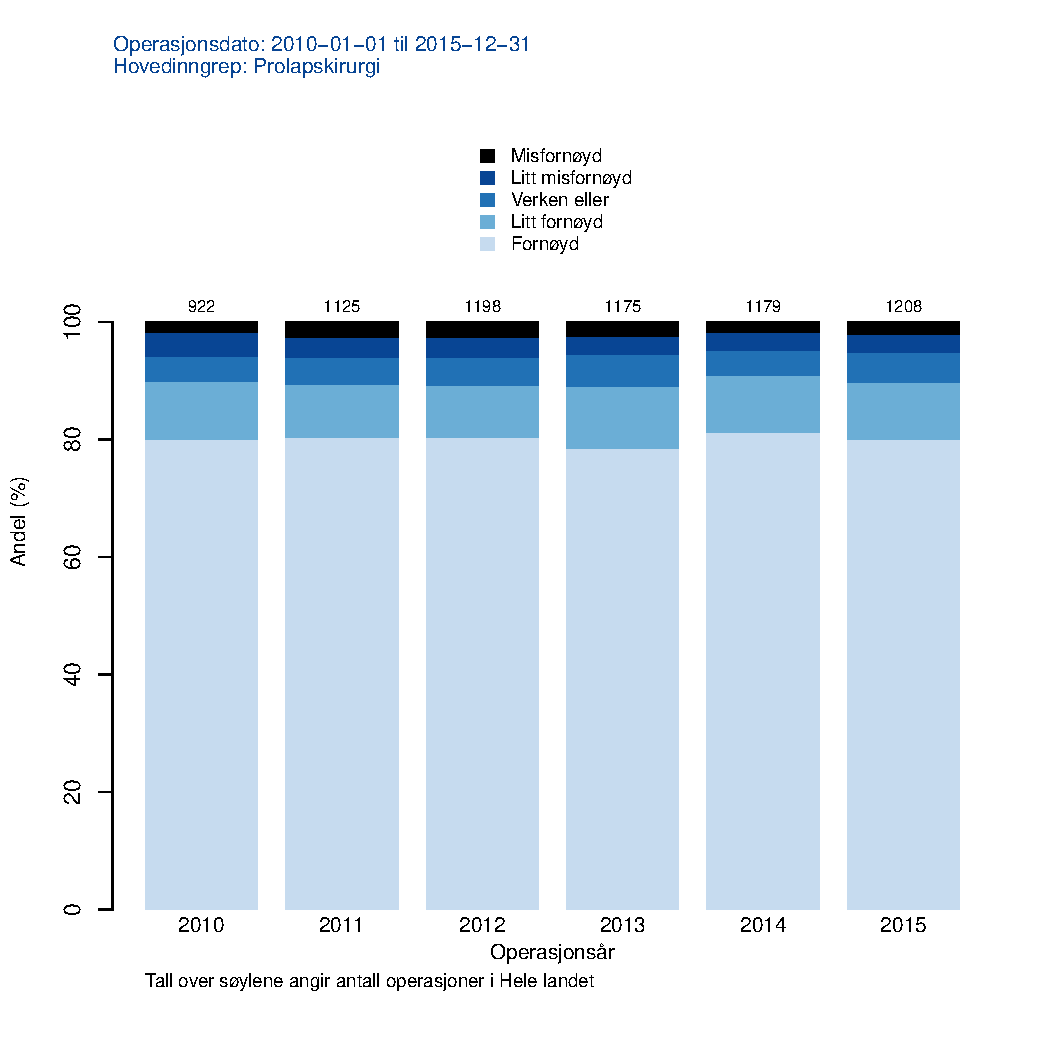
\includegraphics{FigFornoydPro.pdf}}
\scalebox{0.5}{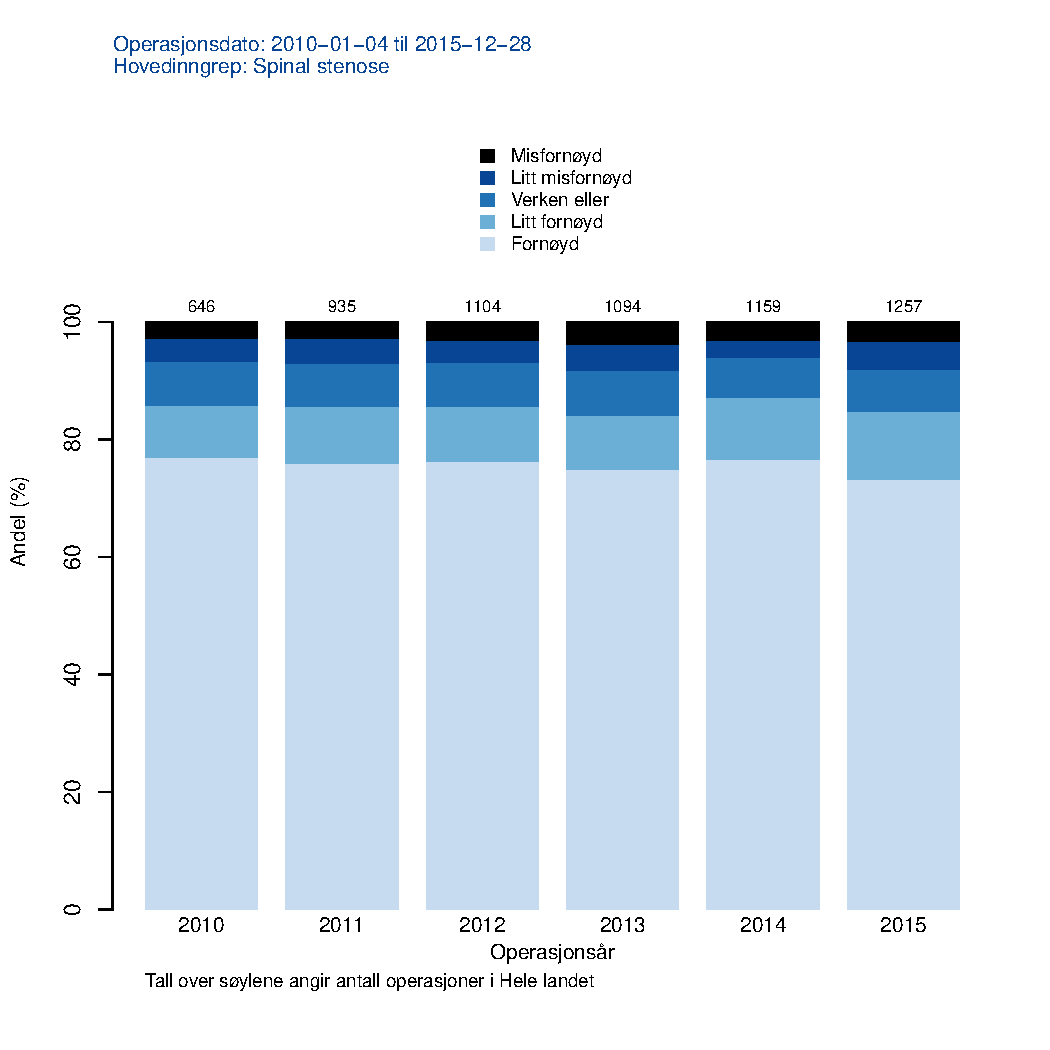
\includegraphics{FigFornoydSS.pdf}}
	\end{center}
  \caption{Spørsmål stilt 12 måneder etter operasjon: Hvor fornøyd er du med behandlinga du har fått på sykehuset?}
  \label{fig:Fornoyd}
\end{figure}





\textbf{Her starter det som i årsrapporten var etter samlerapporten.}




\subsection{ Resultater etter rygg og nakkekirurgi nasjonalt og per sykehus fra 2010 til \Sexp{aar}}

\textit{Følgende avsnitt er ikke oppdatert}

Hyppigst utførte inngrep er for prolaps, dernest for trang ryggkanal (spinal stenose),
dernest mer omfattende avstivningskirurgi (fusjon) for mer komplekse og
sammensatte tilstander. Gjennomsnittlig ODI score var 46 før operasjon og 17 ett år etter
operasjon. Dette betyr at funksjonssvikten ble redusert fra alvorlig til minimal for
gjennomsnittspasienten. \\
Pasienter operert for spinal stenose fikk også
betydelig bedring (ODI redusert fra 41 til 23), men mange har fortsatt moderat
funksjonssvikt ett år etter kirurgi. De som ble operert med fusjon har
omtrent samme forbedring (ODI redusert fra 43 til 26). Dette betyr at selv om
pasientene kan forvente en betydelig bedring, vil mange fortsatt ha moderate restplager
ett år etter kirurgi. Resultatene synes å være stabile over tid. NKR
sammenstiller nå norske resultater med data fra tilsvarende registre i Sverige og
Danmark. Foreløpige analyser tyder på at resultatene er de samme i
de tre nordiske landene.
Resultatene varierer imidlertid mye fra pasient til pasient og mellom sykehus.
Viktige årsaker til variasjon i operasjonsresultat er at ulike sykehus dels behandler
ulike pasientgrupper. Viktig for operasjonsresultatet er imidlertid fortsatt
indikasjonsstillingen («inngangsbilletten») til kirurgi; Fikk riktig person, rett
behandling til rett tid?

Forekomst av risikofaktorer blant pasientene påvirker operasjonsresultatene og kan
si noe om hvor godt behandlingstilbudet fungerer på ulike sykehus. Noen av disse
faktorene kan modifiseres/bedres gjennom bedre styring og planlegging av
virksomheten, strengere indikasjonsstilling og bedret pasientsikkerhet.
Kvalitetsindikatorer


\subsection{Prolapskirurgi (alle kategorier)}



Liggetiden på sykehus i forbindelse med prolapsoperasjon har gått ned med 0.5 døgn fra 2010 til 2016.



\begin{figure}[ht]
	\centering 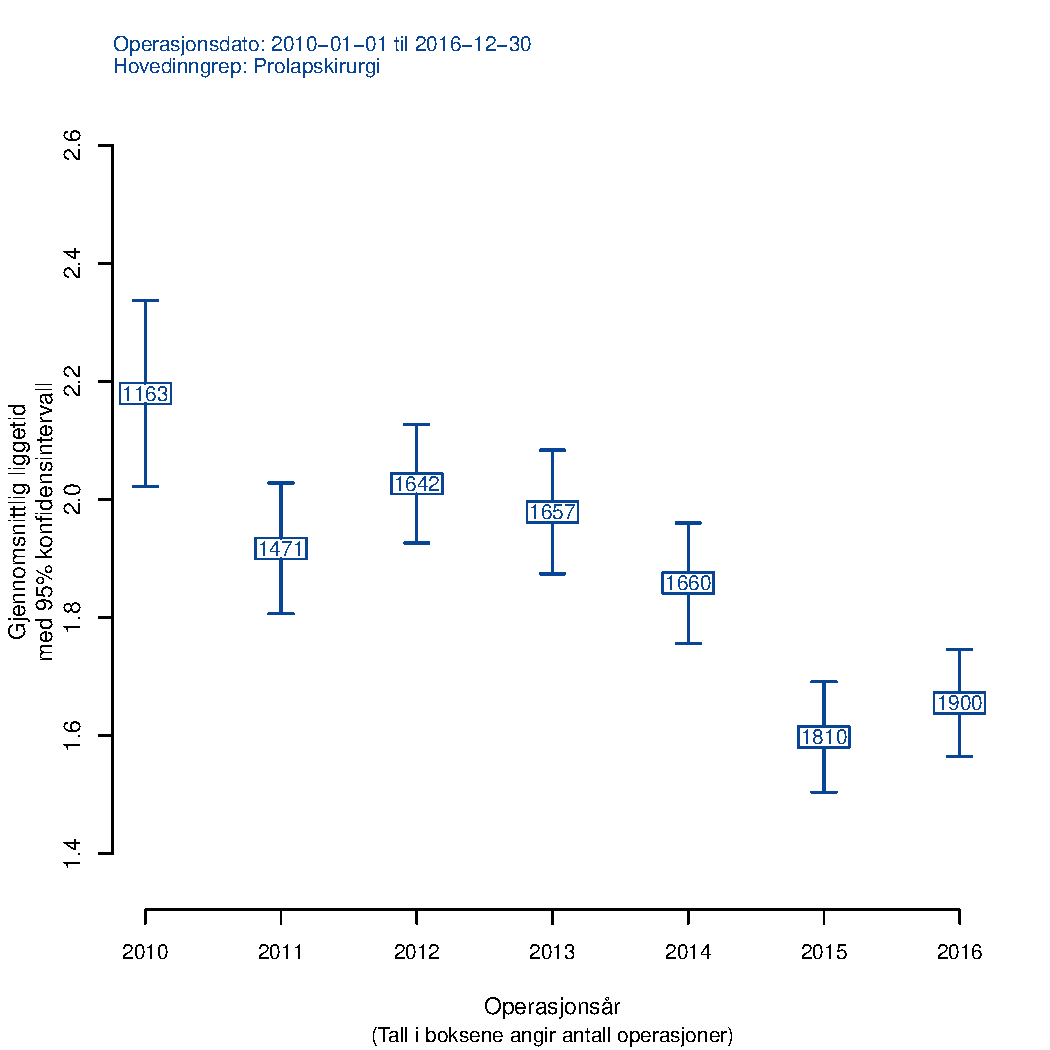
\includegraphics[width= 0.8\textwidth]{LiggetidProlaps.pdf}
	\caption{\label{fig:LiggetidPro} Gjennomsnittlig liggetid per år for pasienter operert for prolaps.}}
\end{figure}


\subsection{Kvalitetsindikatorer}

\textbf{Kanskje si noe om hvordan kvalitetsindikatorene er utarbeidet?}
\begin{knitrout}
\definecolor{shadecolor}{rgb}{0.969, 0.969, 0.969}\color{fgcolor}\begin{kframe}
\begin{verbatim}
##    
##          2010      2011      2012      2013      2014
##   0 13.252094 12.726138  7.035176  1.437258  1.084011
##   1 86.747906 87.273862 92.964824 98.562742 98.915989
##    
##          2015      2016
##   0  1.001502  1.373222
##   1 98.998498 98.626778
##    
##          2010      2011      2012      2013      2014
##   1 80.043384 80.355556 80.300501 78.522920 81.133672
##   2  9.869848  8.977778  8.848080 10.441426  9.644670
##   3  4.121475  4.622222  4.841402  5.517827  4.399323
##   4  4.229935  3.466667  3.422371  3.056027  2.961083
##   5  1.735358  2.577778  2.587646  2.461800  1.861252
##    
##          2015      2016
##   1 80.000000 80.576923
##   2  9.629630  8.653846
##   3  5.267490  6.153846
##   4  3.045267  2.500000
##   5  2.057613  2.115385
\end{verbatim}
\end{kframe}
\end{knitrout}

Andelen som er operert ved hjelp av synsfremmende midler (mikroskop eller
lupebriller), som har åpenbare fordeler, har økt fra 80.8 \% i 2010 til 
98.8 \% i 2016. 

NKR har tidligere vist at multiple reoperasjoner har en minimal og potensiell skadelig
effekt. Andelen som har vært operert mer enn 2 ganger tidligere har gått ned med 1
prosent (fra 5,6 \% i 2010 til 4,5 \% i 2015). 
\textbf{Her har du gjort feil... Du har referert andelen som har >2 tidligere operasjoner av de som har hatt tidligere operasjoner, ikke av alle prolapsoperasjoner. Andelen med >2 tidligere operasjoner ligger i 0.9, 1.5 og er omtrent lik i 2010 og 2016. Jeg har notert at vi skal ha en figur på andel med >2 tidligere operasjoner, men er ikke så sikker på at det er så interessant når andelen ligger så stabilt.}


For alle typer prolapsoperasjoner har
andel sårinfeksjoner (pasientrapportert) har blitt redusert med 1 \% i perioden mens
bruk av forbyggende antibiotikabehandling har økt med 15 \%. 
\textbf{Andelen sårinfeksjon er omtrent lik i 2010 og 2016... Kan evt. ha en figur på andel infeksjon per år... Det er jo en viktig informasjon.}

Andelen
pasienter som er fornøyde med behandlingen de fikk på sykehuset (PREM) har økt
fra 83 til 85 \%. \textbf{Hvordan har du kommet fram til disse tallene...? Andel fornøyde prolapspasienter ligger stabilt rundt 80 \% med 78,5 \% i 2013 og 81,1 \% i 2014.}


\subsubsection{Sykehusvise resultater}



Resultater for planlagt, første gangs prolapsoperasjon i 2016 er vist
nedenfor. Kun avdelinger med mer enn 10 registrerte operasjoner i er med i
analysen. Grunnen til at gjentatt kirurgi (reoperasjon) og øyeblikkelig hjelp (ø-hjelp)
er filtrert bort er at dette er ulikt fordelt mellom sykehusene.

\HUGE{Resten er ikke oppdatert!}

Hos pasienter operert som ø-hjelp er andelen med betydelig forbedring
(suksessraten) 82 \%, mot 62 \% av de som blir operert planlagt (elektivt).
Hos de som ikke har vært operert i ryggen tidligere er suksessraten 66 \% mot 60\%
hos de som reopereres. Dersom man har vært operert mer enn 2 ganger tidligere i
ryggen faller suksessraten til 38 \%. Sykehus får henvist få pasienter som ø-hjelp og
mange til reoperasjon vil dermed få dårligere resultater.






\subsubsection{God indikasjonsstilling (rett pasient)}

Pasienter som har mye plager, vil kunne forvente størst nytte av ryggoperasjon,
mens de som har lite plager vil ha mindre potensial for forbedring og større risiko
for forverring. Gevinst av kirurgi henger derfor sammen med hvor streng
indikasjonsstillingen («inngangsbilletten» til kirurgi) har vært. Figur 8 viser denne
sammenhengen tydelig. Verdt å merke seg er at hvis pasienten har lite smerter før
operasjon (bensmerter under ca. 2,5 på den horisontale smerteskalaen), er det stor
sjanse for at pasienten faktisk blir verre (negativt tall på den vertikale skalaen) etter
operasjon. Figur 9 viser at det er stor variasjon i hvor stor grad sykehusene opererer
pasienter med prolaps og lite bensmerter. Pasienter med lammelse (parese) er tatt
ut av analysen, da de ofte må opereres uansett grad av smerte.

\textit{tekst flyttes?}


Figur 3.11: Sammenheng mellom intensitet av bensmerte før operasjon og
forbedring etter operasjon. Skala for bensmerter går fra 0 til 10, hvor 0 betegner
ingen og 10 verst tenkelige smerte før operasjon (horisontal akse). Negativ endring
av bensmerten (vertikal akse) tilsvarer forverring, 0 betyr uendret smerte etter
operasjon.

Figur 3.12: Andel pasienter med lite bensmerter (under 2,5) operert for prolaps ved
norske sykehus.


\subsubsection{Resultatindikatorer (behandlings-effektivitet)}
Viktige tiltak for å bedre behandlingseffektivitet vil være å øke andelen som får en
betydelig forbedring (suksessraten), redusere andelen som ikke har nytte av
behandlingen, blir verre eller får komplikasjoner. Nedenfor vises noen indikatorer
(«bench-mark kriterier») som NKR har utviklet og validert for
behandlingseffektivitet sammen med forekomst av de hyppigste komplikasjonene.
Forskjellene skyldes dels at pasientgruppene som opereres ved ulike sykehus har
- Side 20 -
ulik risikoprofil. Resultatene som vist i figurene nedenfor er ikke justert for disse
forskjellene. Kunnskap om risiko kan dette bidra til bedre utvelgelse av pasienter til
kirurgi.


\subsubsubsection{Uønsket resultat II}

Pasienter som 1 år etter prolapskirurgi har en ODI skår over 48 har fortsatt alvorlig
smerterelatert funksjonshemming i dagliglivet. Flesteparten av disse pasientene vil
oppfatte sin livssituasjon for klart verre enn før operasjonen.
Figur 3.14: Andel pasienter med alvorlig smerterelatert funksjonssvikt 1 år etter
prolapskirurgi.


\subsubsubsection{Uønsket resultat III}
Pasienter med forbedring av ODI skår mindre enn 13 vil som hovedregel ikke
oppfatte sin situasjon som vesentlig forbedret etter kirurgi. Resultatet blir dermed å
betrakte som utilfredsstillende.
Figur 3.15: Andel pasienter som ikke oppnår et tilfredsstillende resultat, ODI
forbedring >13 etter prolapskirurgi.


\subsubsubsection{Ønsket resultat («suksess»)}
Figur 3.16: Andel pasienter med betydelig forbedring av selvrapportert
smerterelatert funksjon i dagliglivet («suksess», ODI forbedring over 20 poeng) 1 år
etter prolapsoperasjon.

\subsubsubsection{Komplikasjoner (sikkerhet)}
I. Sårinfeksjon.
Årsakene til sårinfeksjon er komplekse. I 2016 fikk 98-100 \% av pasienter som
opereres for prolaps forebyggende antibiotikabehandling under operasjon. NKR
viste for mange år siden at dette har god forbyggende effekt.
Figur 3.17: Andel pasienter som rapporterer om sårinfeksjon 3 måneder etter
prolapskirurgi.


\subsubsubsection{II. Durarift (rift på ryggmargshinnen)}
III.
Dette er oftest en ufarlig komplikasjon, men kan medføre væskelekkasje og
ubehag for pasienten, lengre liggetid og i noen tilfeller behov for reoperasjon.
Unntaksvis kan også nerveskade og alvorlig infeksjon forkomme.
Figur 3.18: Andel pasienter som får durarift etter kirurgi for prolaps
(primæroperasjon, elektiv).


Andre faktorer som varierer mellom sykehus og kan påvirke resultatene
Andelen fremmedspråklige som opereres for prolaps har økt fra 5 til 7 \% i perioden.
Beslutning om ryggkirurgi baserer seg på en felles forståelse mellom kirurg og
pasient av hva helseproblemene består i og hva som kan oppnås med operasjon
(«shared desicion making»). I behandling av fremmedspråklige er kommunikasjon
en utfordring. Av de som har norsk som morsmål var suksessraten 65 \% mot 56 \%
for fremmedspråklige. Bedre kommunikasjon kan bidra å redusere disse
forskjellene.
Figur 3.19: Andel fremmedspråklige av alle prolapsopererte ved ulike sykehus i
Norge.


\section{Resultater degenerativ nakke}
I Norge drives nakkekirurgi kun ved nevrokirurgiske avdelinger knyttet til de fem
universitetssykehusene i Oslo, Bergen, Trondheim, Stavanger og Tromsø, samt ved
hovedsakelig ett privat sykehus (Oslofjordklinikken).
Da der ikke finnes etablerte kvalitetsindikatorer for nakkekirurgi vil dette bli en
viktig oppgave for NKR. Da en ny validering av datakvaliteten ikke er fullført grunnet
uventede databaseproblemer, vises kun et generelt mål på pasient rapporterte
tilfredshet (PREM) i årets rapport. I neste årsrapport vil NKR presentere sykehusvise
kvalitetsdata splittet på diagnose, behandling.
Pasienttilfredshet (PREM)
Her har pasienten svart på hvor fornøyd de var med behandlingen de fikk på
sykehuset. Dette er et lite spesifikt effektmål som gir uttrykk for totalopplevelsen,
det vil si mange aspekter knyttet til både informasjon, utredning, opphold,
behandling og oppfølging.
Figur 3.20: Andelen nakkeopererte som fornøyde med behandlingen ved Norske
sykehus 12 måneder etter nakkekirurgi.
- Side 28 -
Pasienter som opereres i nakken for degenerative tilstander har armsmerte med
eller uten funksjonssvikt (radikulopati), varierende grad av nakkesmerter og noen
har ryggmargspåvirkning (myelopati). Som hovedregel kan ikke pasienter som
opereres på grunn av ryggmargspåvirkning påregne bedring i samme grad som de
som behandles for armsmerte. Figur 3.21 viser at også andelen som opereres for
myelopati varierer mellom sykehusene.
Figur 3.21: Andel pasienter som opereres for ryggmargspåvirkning (myelopati) ved
norske sykehus.
- Side 29 -
3.3 Oppsummering av de viktigste resultatene
- Dekningsgraden er fortsatt under 80 \%, men økende.
- Innen offentlig helsetjeneste synes kvalitetssikring av egen virksomhet å
være høyt prioritert på Sørvest-landet og i Sør-Trøndelag, men ikke i Helse
Sørøst og Møre & Romsdal HF.
- Ryggopererte opplever generelt en sterk, klinisk relevant og statistisk
signifikant forbedring av funksjon i dagliglivets aktiviteter, livskvalitet og
arbeidsuførhet. Resultatene er stabile over tid.
- Liggetiden er fortsatt redusert i 2016. Dette kan knyttes til økt bruk av
mindre omfattende kirurgi.
- Bruke av synsfremmende midler under operasjon øker
- Andelen pasienter som er fornøyde med behandlingen de fikk på sykehuset
12 mnd. etter operasjon øker blant prolapsopererte, og andel multiple
reoperasjoner og andel sårinfeksjoner går ned. Andel som har søkt
uføretrygd før operasjon er redusert. Andelen pasienter med lang
symptomvarighet før operasjon er ikke redusert.
- Det er stor variasjon i resultat mellom sykehus
- Strengere indikasjonsstilling vil kunne bedre operasjonsresultatene
- Pasienttilfredsheten blant nakkeopererte varierer mellom 80-90 \% ut fra
hvor pasientene er operert og type diagnose.









\end{document}
